\begin{frame}[plain]
  \begin{tikzpicture}[remember picture,overlay]
    \node[at=(current page.center)] {
      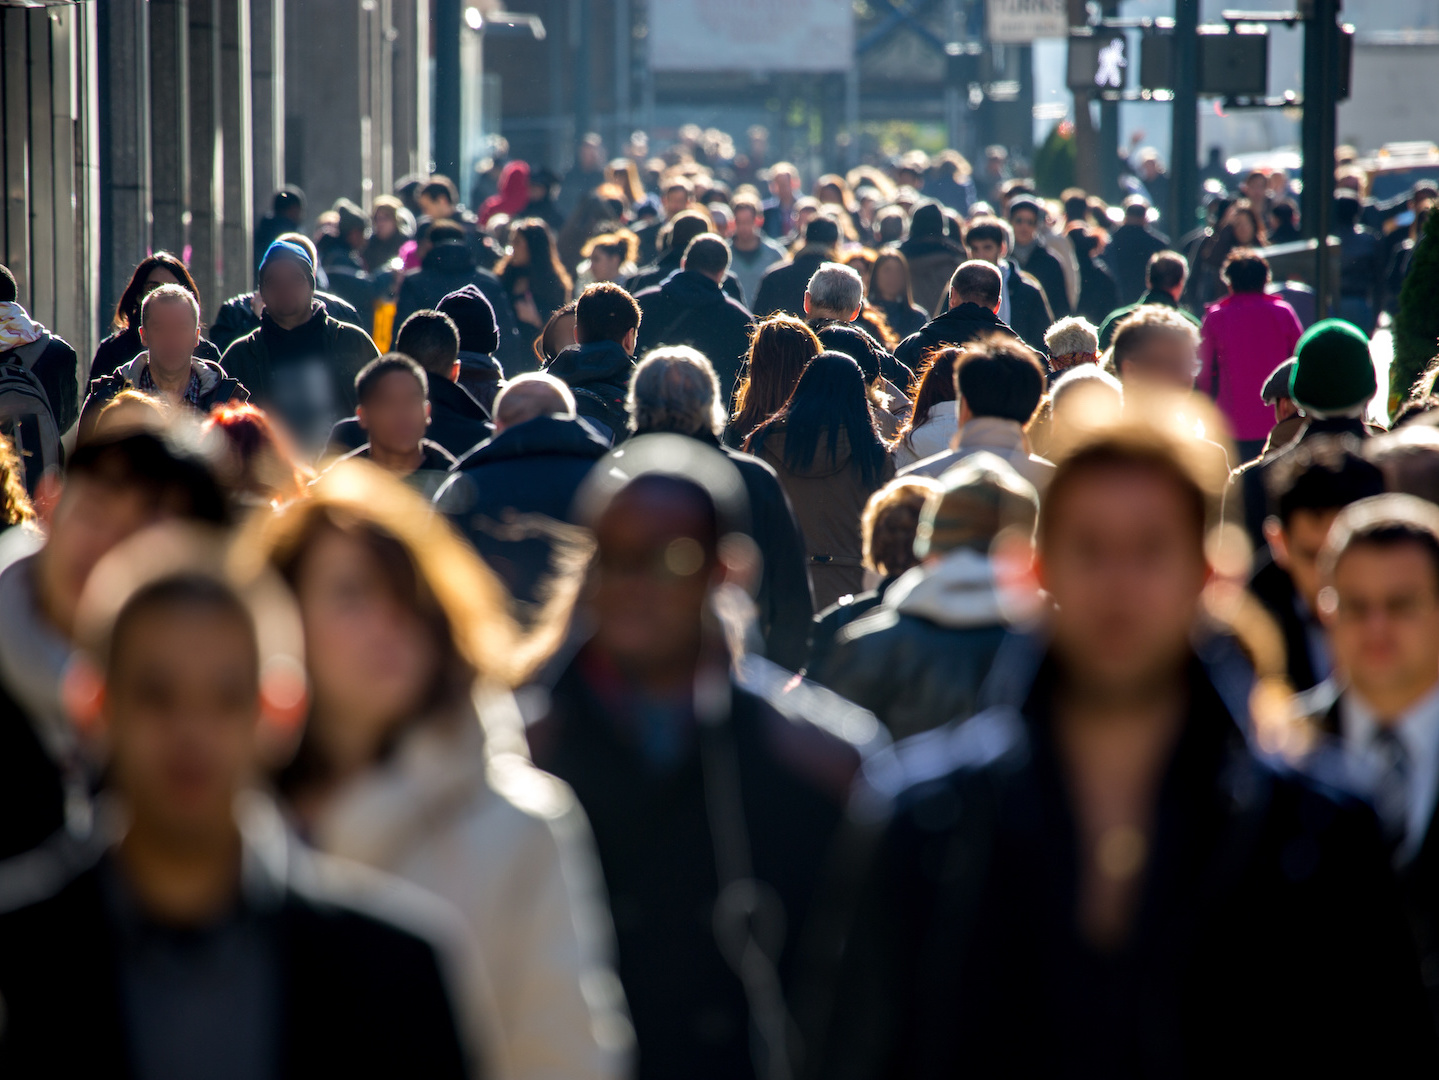
\includegraphics[width=\paperwidth]{crowd_street.jpg}
    };
  \end{tikzpicture}
\end{frame}

\section{Partial Occlusion Handling}
\label{sec:Partial Occlusion Handling}


\begin{frame}{Partial Occlusion Handling}
\small
\metroset{block=fill}

  \begin{alertblock}{\textbf{Why?}}
  Generally, especially in crowded scenes, occlusions occur frequently.
  Nevertheless, generic detectors, such as HOG, assume that pedestrians are fully
  visible and their performance degrades when pedestrians are partially occluded.
  \end{alertblock}
\pause

  \begin{exampleblock}{\textbf{How?}}
  The key to successful detection of partially occluded pedestrians is to use additional
  information about which body parts are occluded, for example \textit{correlations among
  the visibilities of different parts} having different sizes.
  \end{exampleblock}

\end{frame}


\begin{frame}{Partial Occlusion Handling}
  \metroset{block=fill}
  \begin{alertblock}{Probabilistic Framework}
    It models correlations among the visibilities of parts as hidden variables
  \end{alertblock}

\pause

  \begin{exampleblock}{Deep Model}
    The hierarchical structure of the deep model matches with the multilayers of
    the parts model well.
    Different from the other types of deep networks, whose hidden variables had
    no semantic meaning, this model considers each hidden variable as representing
    the visibility of a part.
  \end{exampleblock}

\end{frame}


\begin{frame}{A little bit of math}

Let $\mathbf{x}\in\mathbb{R}^d$ and $y\in\lbrace0,1\rbrace$ be respectively the \textit{feature vector} and the \textit{label} of a detection window.\\
\vspace{3mm}
\pause
Denote the detection scores of the $P$ parts by $\mathbf{s} = [s_1,...,s_P]^T = \gamma(\mathbf{x})$, where $\gamma(\mathbf{x})$ are part detectors.\\
\vspace{3mm}
\pause
Denote the visibilities of the $P$ parts by $\mathbf{h} = [h_1,...,h_P]^T \in\lbrace0,1\rbrace^P$, with $h_i = 1$ meaning \textbf{visible} and $h_i = 0$ meaning \textbf{invisible}.

\end{frame}


\begin{frame}{Hidden variable framework}
\begin{equation}
  p(y\vert\mathbf{x}) = \sum_\mathbf{h}p(y,\mathbf{h}\vert\mathbf{x}) = \sum_\mathbf{h}p(y\vert\mathbf{h},\mathbf{x})p(\mathbf{h}\vert\mathbf{x})
\end{equation}

%\pause
%  Often, for a fast approximate solution, this relation is simplified as follows:
%\begin{equation}
%  p(y\vert\mathbf{x}) \approx \exp \left( \sum_i s_i \right)
%\end{equation}

\pause
\metroset{block=fill}
\begin{block}{Objective}
  Build a deep model that learns the correlation of visibility
   relationship among parts
\end{block}

\end{frame}

\begin{frame}{Deep Model for Part Visibility Estimation}
\centering
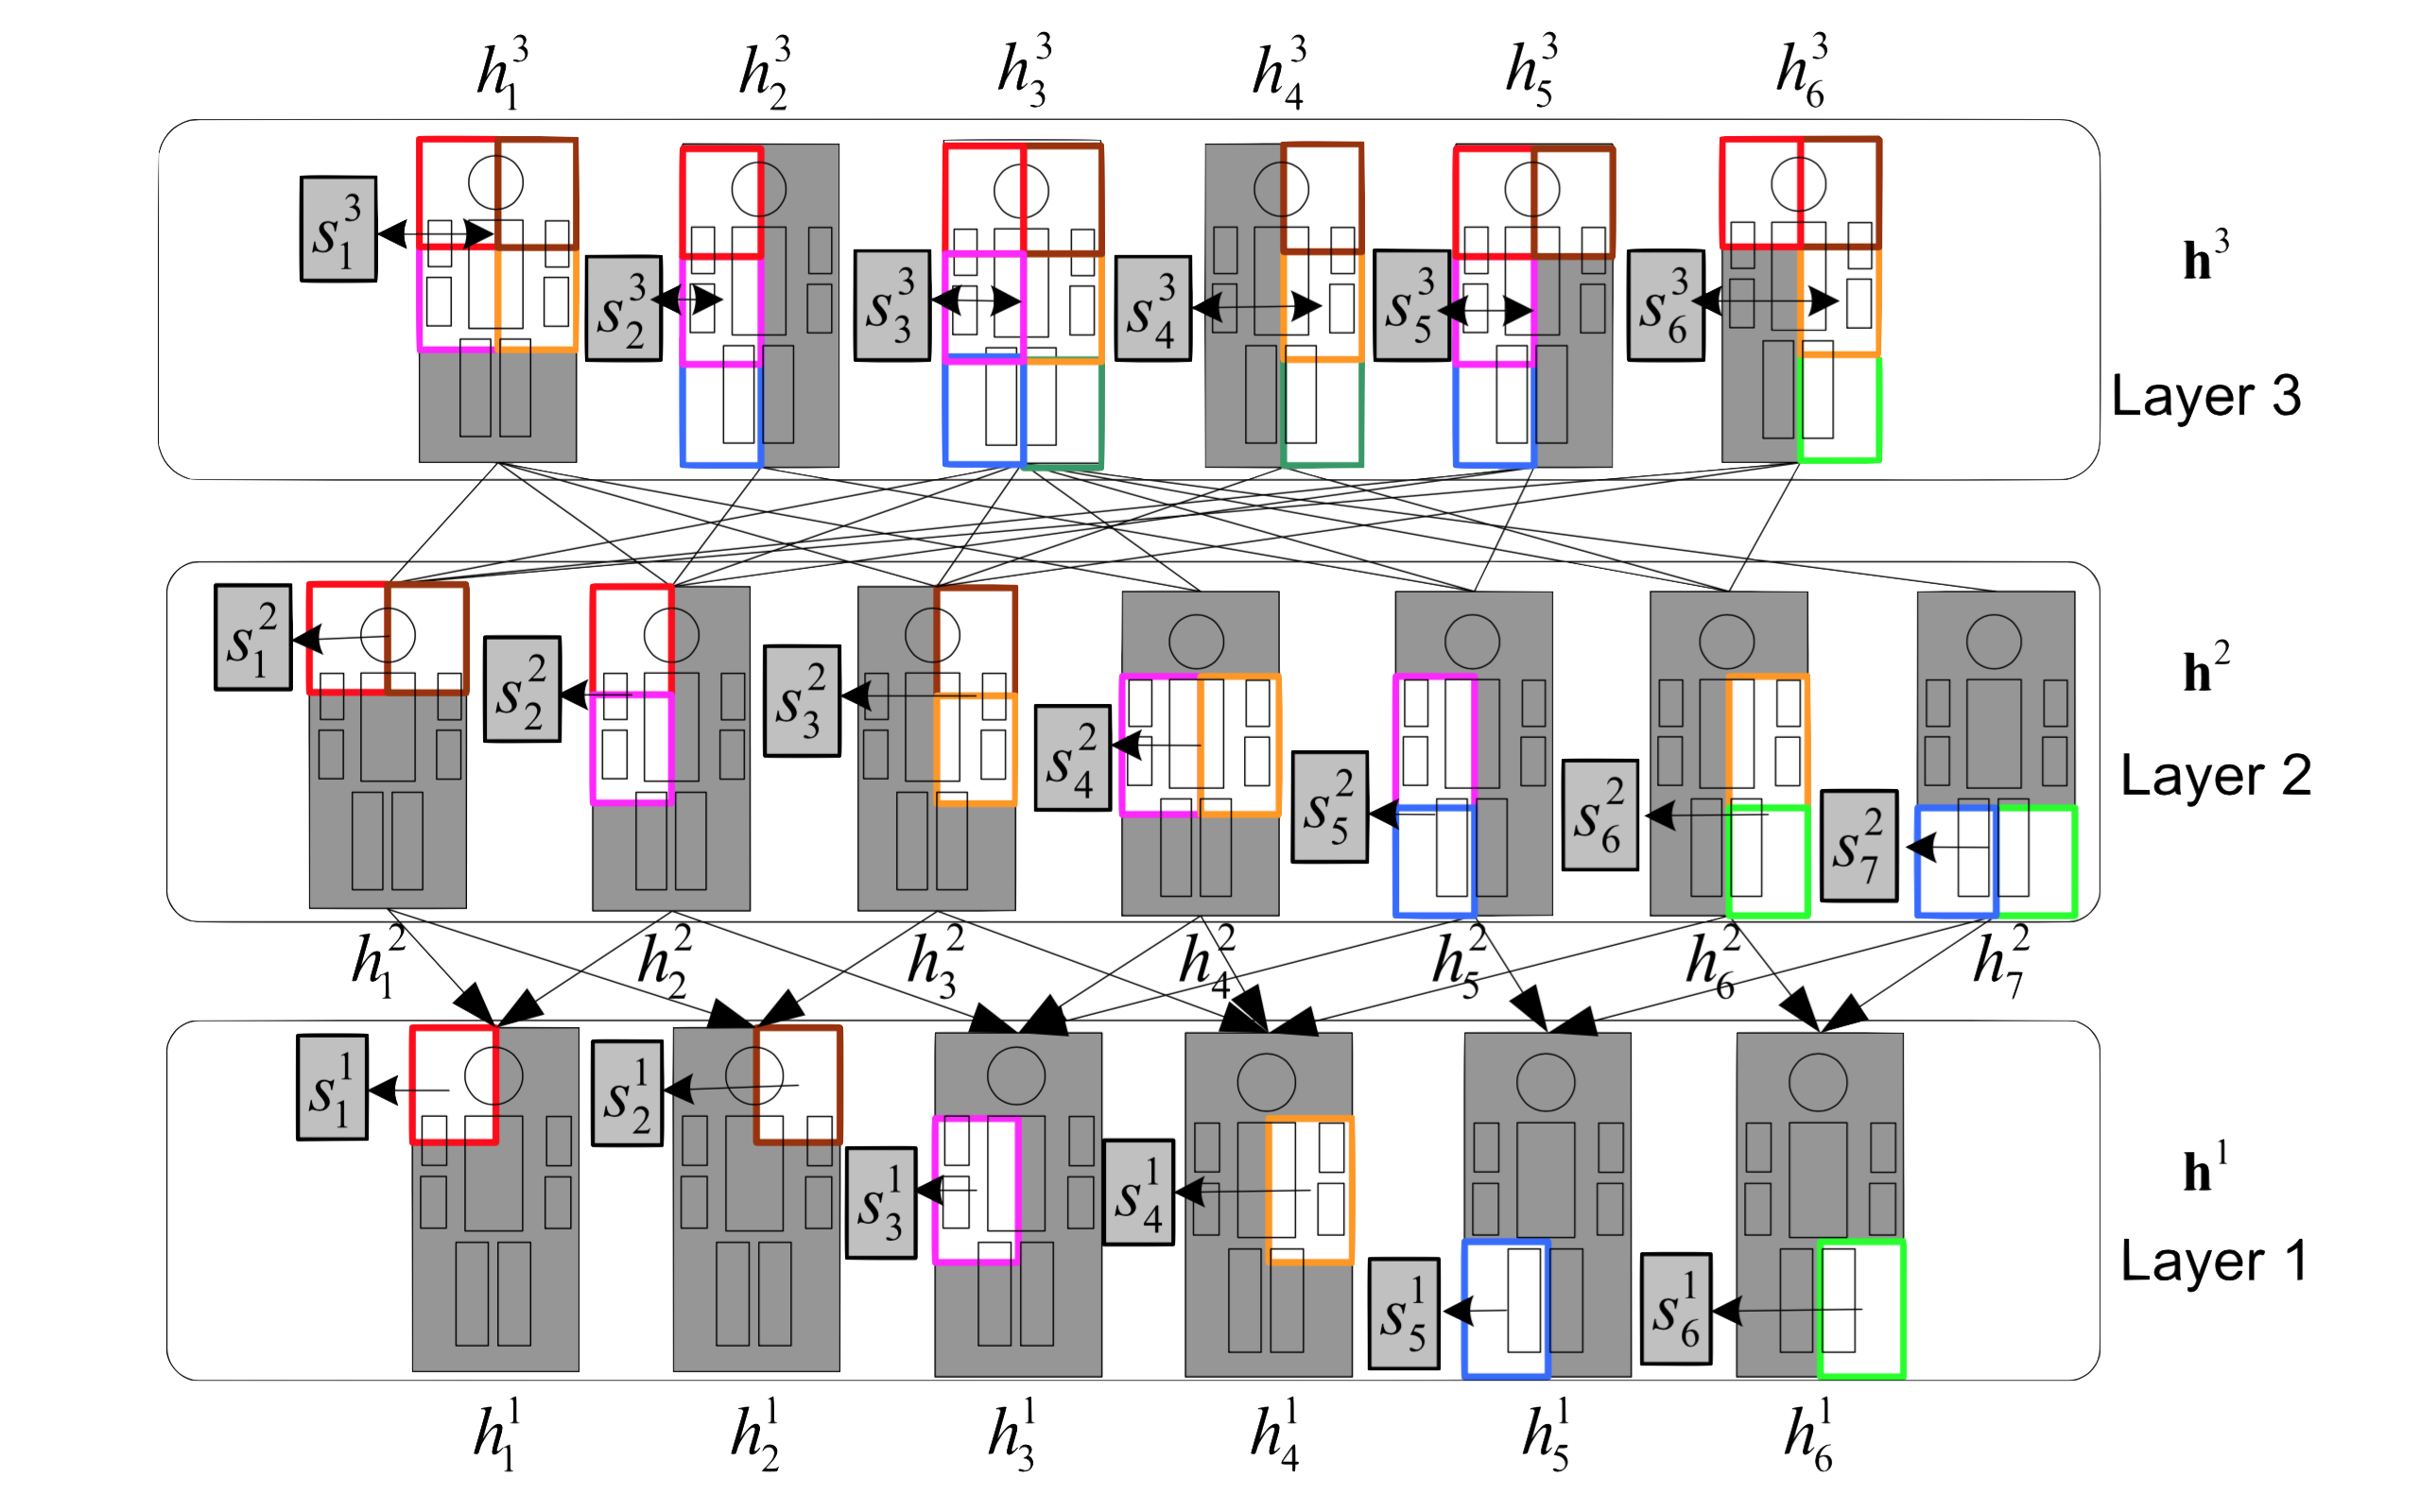
\includegraphics[width=0.85\textwidth]{mlp2.png}
\\
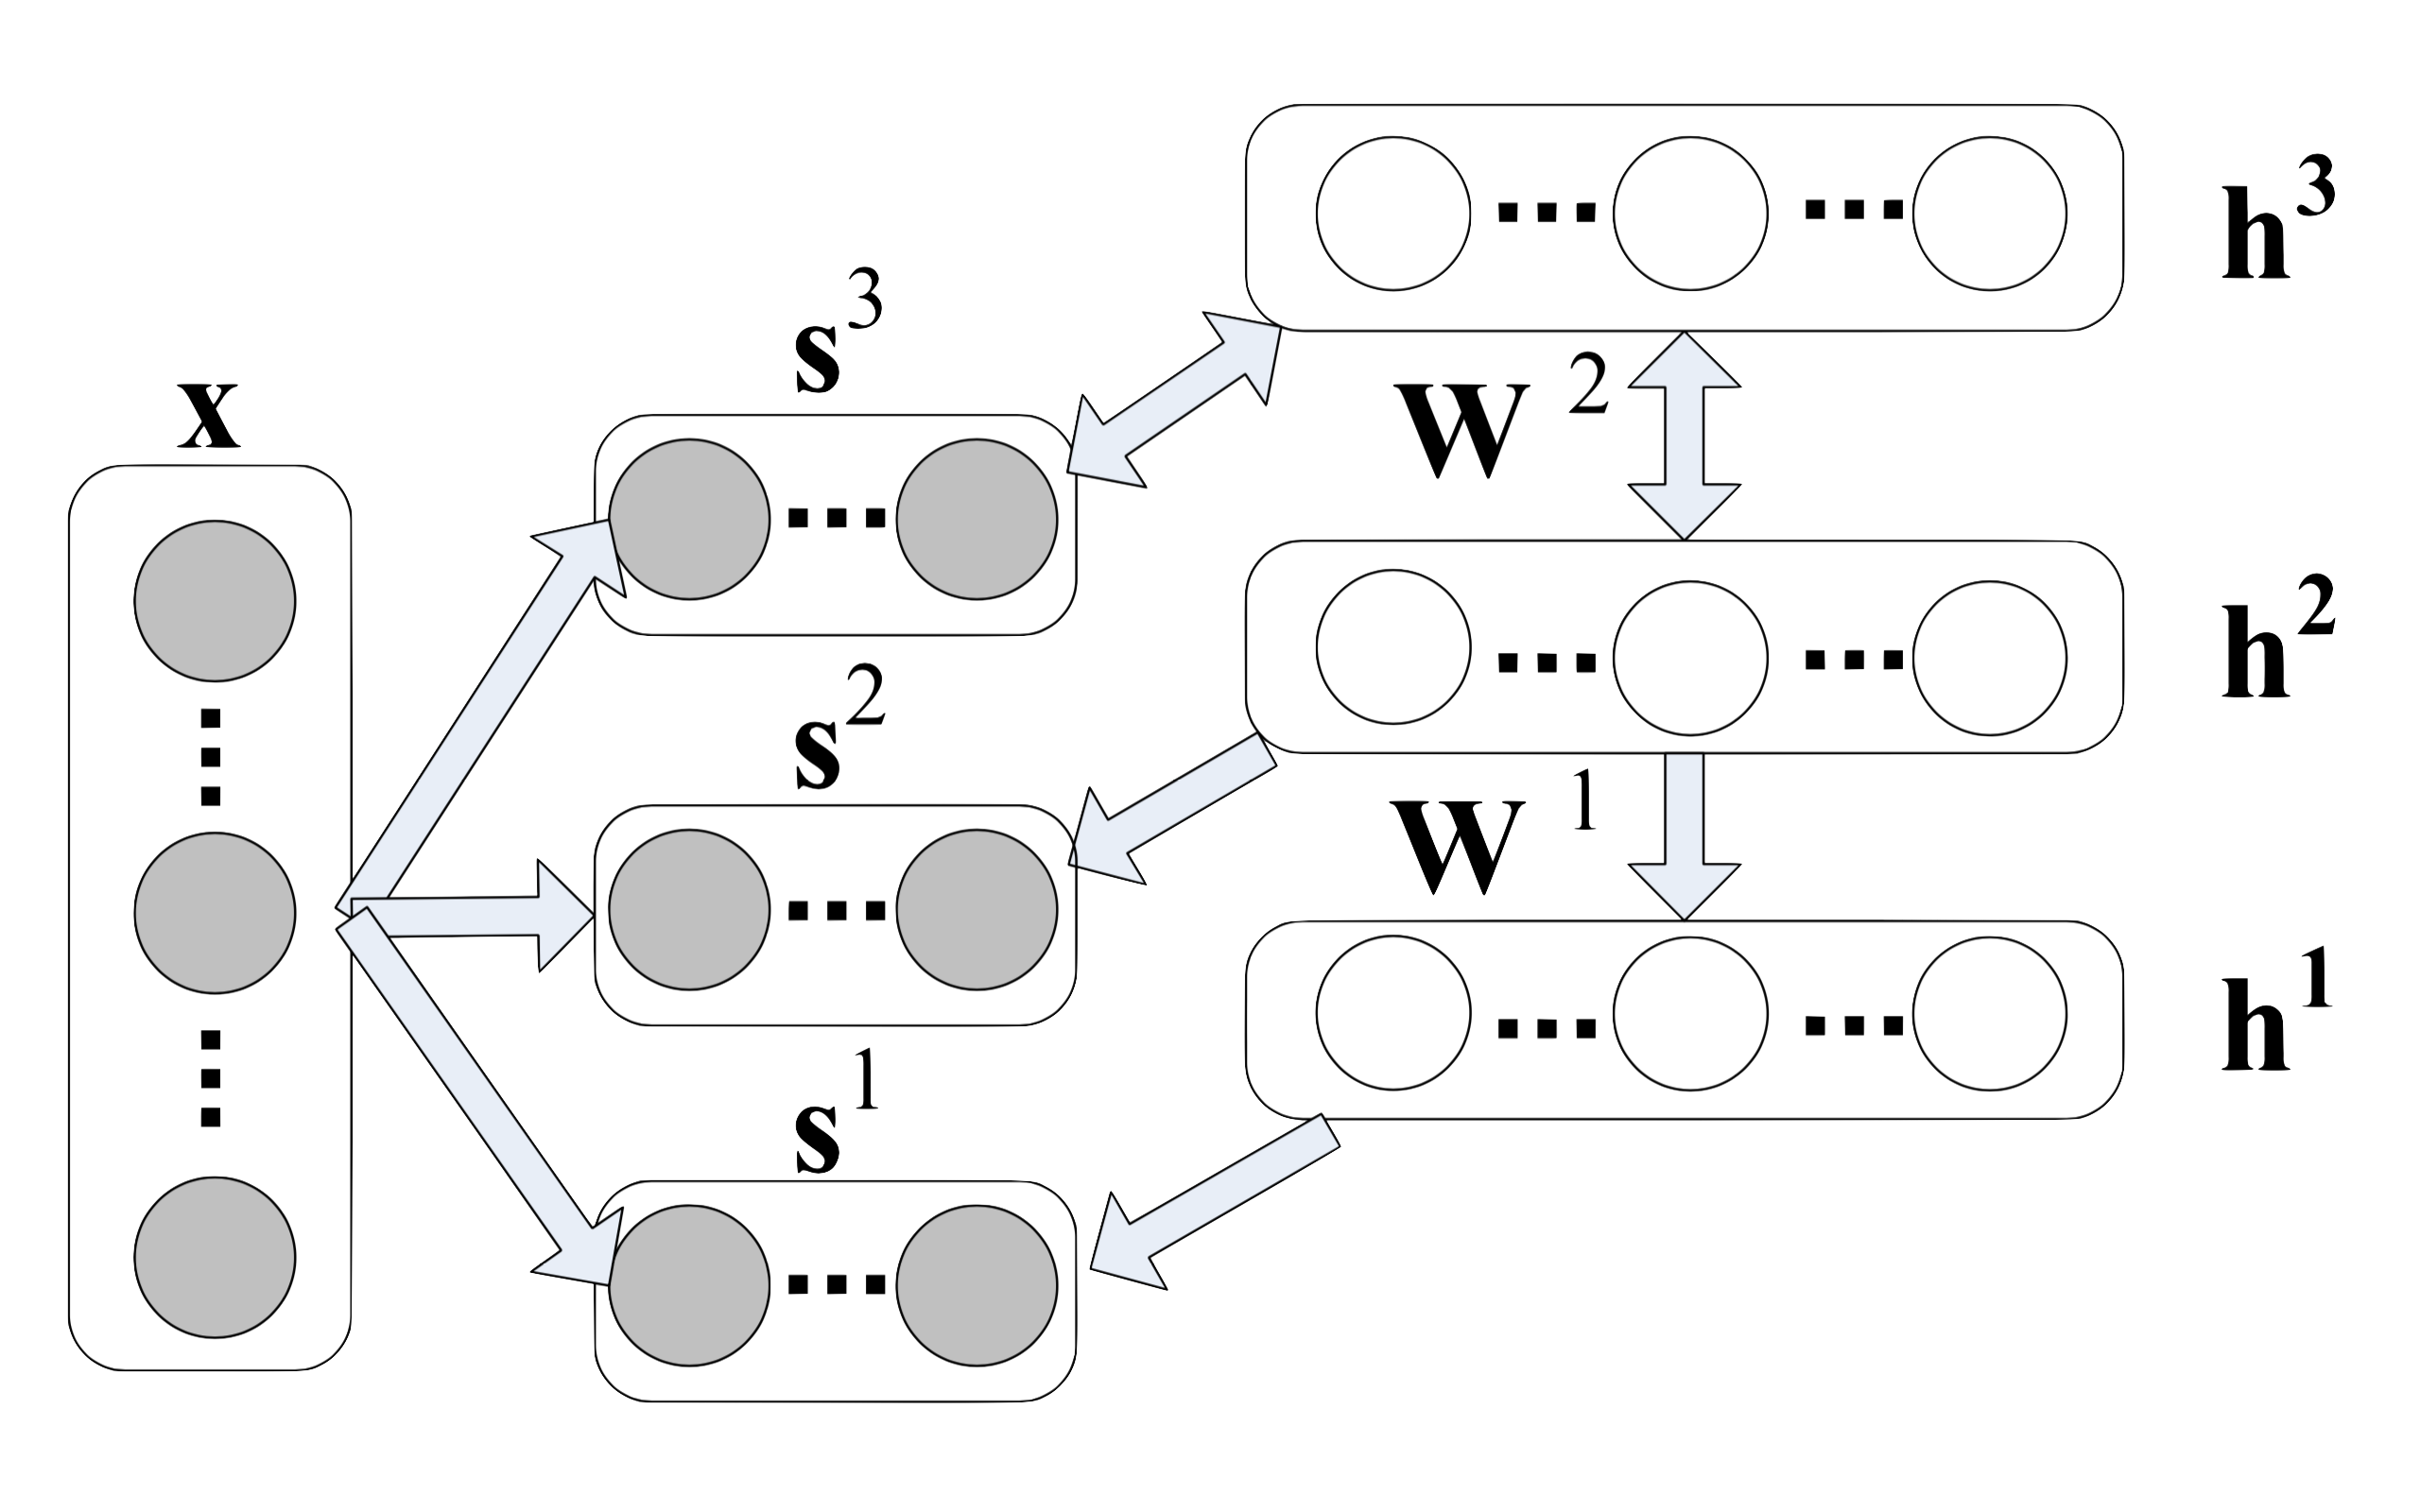
\includegraphics[width=0.3\textwidth]{mlp1.png}
\end{frame}

\begin{frame}{Result}
  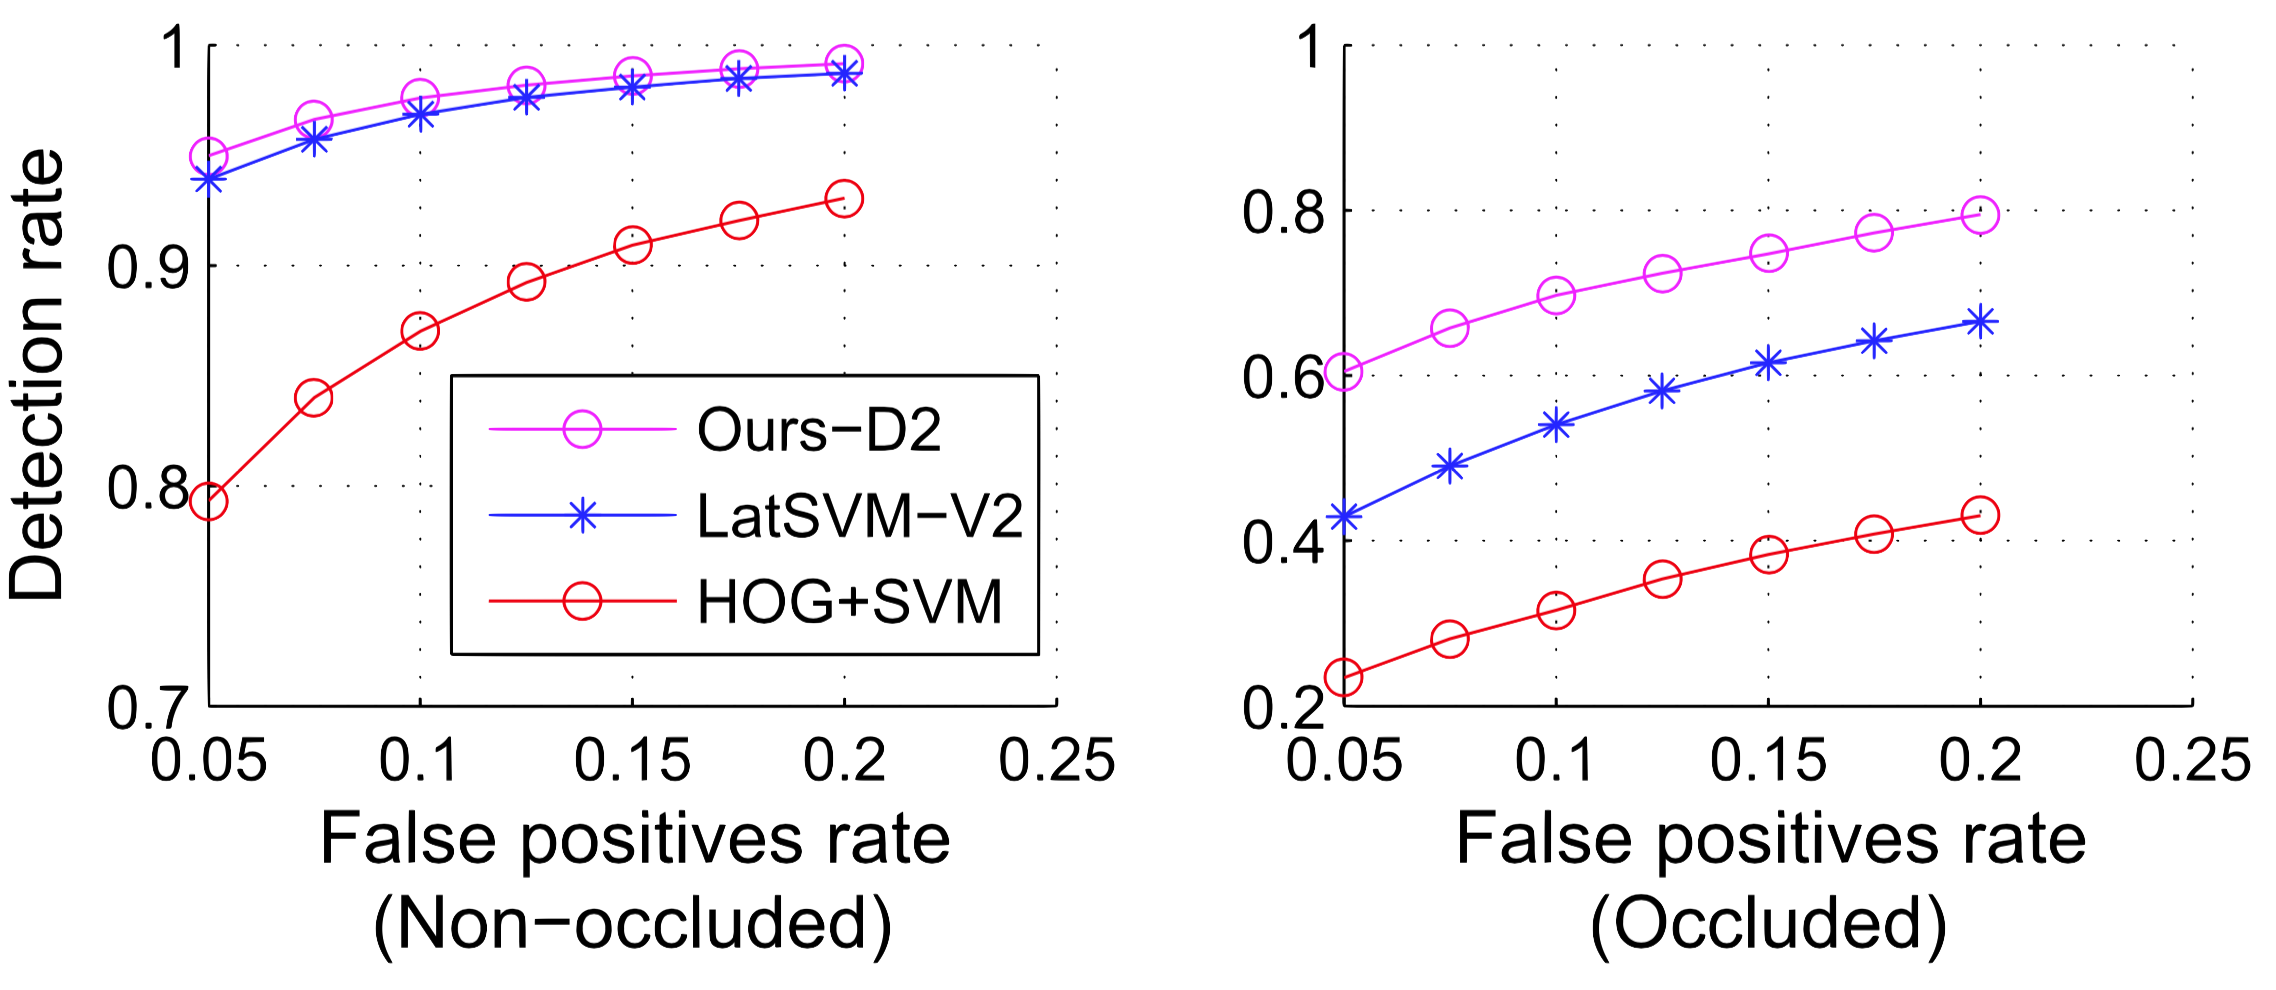
\includegraphics[width=\textwidth]{mlp_result.png}
\end{frame}
